\documentclass[journal]{IEEEtran}
\usepackage{blindtext}
\usepackage{graphicx}

\ifCLASSINFOpdf

\else

\fi


% correct bad hyphenation here
\hyphenation{op-tical net-works semi-conduc-tor}


\begin{document}

\title{Motor speed control of titanium tape using bluetooth and a pulsed x-ray table-top source}


\author{Henrique~VICENTE~SOUZA,~Undergraduate~Student~UNICAMP-University~of~Campinas,\\
        and~Davi~RODRIGUES,~Undergraduate~Student~UNICAMP-University~of~Campinas.%,\\
        %and~George~Nicolas~KONTOGIORGOS,~Undergraduate~Student~UNICAMP-University~of~Campinas.% <-this % stops a space
        
\thanks{Henrique~VICENTE~SOUZA is a last-year's Undergraduate Student at UNICAMP-University of Campinas in Automation and Control Engineering, located in Campinas, S\~{a}o Paulo, Brazil. Henrique has successfully finished a Bachelor (BSc) of Engineering with major in Mechatronics, and a Master (MSc) of Engineering with major in Systems Engineering, Robotics and Embedded Systems, in a Double Degree Program at ENSTA-ParisTech, located in Paris, France. Contact by the e-mails: henriquevs.br@gmail.com, and h105063@dac.unicamp.br.}% <-this % stops a space

\thanks{Davi RODRIGUES is an Undergraduate Student at UNICAMP-University of Campinas in Automation and Control Engineering, located in Campinas, S\~{a}o Paulo, Brazil. Contact by e-mail: davirdgs@gmail.com.}% <-this % stops a space

% \thanks{George Nicolas KONTOGIORGOS is an Undergraduate Student at UNICAMP-University of Campinas in Electrical Engineering, located in Campinas, S\~{a}o Paulo, Brazil. Contact by e-mail: xxxxxx@yyyy.com.}
}


% The paper headers
% \markboth{Journal of \LaTeX\ Class Files,~Vol.~13, No.~9, September~2014}%
% {Shell \MakeLowercase{\textit{et al.}}: Bare Demo of IEEEtran.cls for Journals}
\markboth{WSEE - ES670 Embedded Systems Workshop,~Vol.~2, June~29,~2016}%
{Shell \MakeLowercase{\textit{et al.}}: Bare Demo of IEEEtran.cls for Journals}



\maketitle

% As a general rule, do not put math, special symbols or citations
% in the abstract or keywords.
\begin{abstract}
%\blindtext[1]
Since the aim of mechatronics is to improve the functionality of technical systems, it may be used to implement a rotation speed control of a titanium tape in an embedded system, in order to capture femtosecond x-ray pulses from a table-top laser source. This embedded system has application in multidisciplinary areas as in biological systems, where structural dynamics of myoglobin can be better understood by the capture of information about the photo-excitation of carbon monoxide, for example. A low cost embedded system may increase accessibility in the use of the information stored in the cells and its chemical and biological reactions concerning, for example, the human body, once the price of the final system would not be too high. Then, the control the titanium tape's rotation speed allows the correctly understanding of interesting phenomena which are found in the sup-picosecond time scales not available for synchrotron techniques, by registering femtosecond x-ray pulses, which means that a refined analysis of unknown info may be made afterwards, impacting positively not only the academic domain by the knowledge acquired, but also the society.
\end{abstract}

% Note that keywords are not normally used for peerreview papers.
\begin{IEEEkeywords}
Femtosecond, Pulsed X-ray, Modeling, Bluetooth, Embedded Systems.
\end{IEEEkeywords}

\IEEEpeerreviewmaketitle

\section{Introduction}

\IEEEPARstart{T}{he} purpose of this paper is to present the embedded system developed to control a mechatronics system used to capture femtosecond x-ray pulses, as a project of the Embedded Systems Laboratory Project Course \cite{IEEEhowto:denis} at "FEM" - Faculty of Mechanical Engineering in partnership with "Gleb Wataghin" Institute of Physics, both at University of Campinas - UNICAMP, Campinas, Brazil. Advanced synchrotron radiation techniques are being developed to obtain refined analysis in materials science, so one particular case of study is devoted to obtain time resolved information using the sub-nanosecond x-ray pulses from bunches of the synchrotron storage ring, allowing to probe picosecond dynamics of systems in multidisciplinary areas. Interesting applications within biological systems are the dynamics of the isomerized cis-trans conformation of rhodopsin found in human eyes, or the structural dynamics of myoglobin by the photo-excitation of carbon monoxide. Unfortunately interesting phenomena is found in the sup-picosecond time scales, which is not available for synchrotron techniques. An interesting complementary tool is the use of a table-top laser based femtosecond x-ray sources being developed worldwide. At UNICAMP a prototype of this source has been developed, where x-ray pulses are produced by the interaction of 1 [mJ], 60 [fs] near infrared pulses focused at a titanium tape target at 1 [kHz] repetition rate.

The implementation is made by using the Kinetis Software Design Studio \cite{IEEEhowto:Kinetis} to test, compile, and build the embedded system. It will be implemented on FRDM-KL25Z4 NXP Board platform \cite{IEEEhowto:FRDM-KL25Z4} and will use C language, as well as libraries provided by NXP. The project is divided by 6 parts, which are highlighted in the following sections.

\section{Project Design}

%Neste capitulo discorreremos sobre como se deu a evolucao da ideia.
In this chapter we discuss how was the evolution of the gerneral idea for this project.

\subsection{Femto before the project}

% O projeto Femto consiste de uma fita alvo de titânio. Ao ser atingidos por fótons de alta velocidade vindos de um laser, o titanio tem eletrons extraidos quando os fotons chocam com seus atomos, causada pela rapida desaceleracao dos fotons de laser. Este processo desencadeia a geracao de raio-x atraves do fenomeno de Bremmsstrahlung \cite{IEEEhowto:Bremmsstrahlung}. O objetivo do projeto e gerar feixes de raio-x pulsado utilizando para tanto uma fonte pulsada de raio-x.

The Femto project consists of a target tape of titanium. On being hit by high-speed photons coming from a laser, the titanium extracts electrons when photons collide with their atoms, caused by the rapid deceleration of the laser photons. This process triggers the x-ray generation through the phenomenon of Bremmsstrahlung \cite{IEEEhowto:Bremmsstrahlung}. The project's objective is to generate pulsed x-ray beam using a pulsed laser source.

% Ao se chocar com os fotons de laser, o titanio se degrada. Sendo assim e necessario que o titanio seja constantemente reposto na frente do laser. Para tanto se utiliza um sistema de fitas, onde dois motores DC \cite{IEEEhowto:motor} enrolam o titanio, mantendo uma velocidade tangencial constante. Como o foco do laser é muito pequeno (20 $\mu m$), vibrações na fita nao sao toleradas pelo sistema, pois o foco do laser deve insidir exatamente sobre a fita.
% Para controle do motor era utilizado o modulo C-863 da PI \cite{IEEEhowto:PI}.

When colliding with laser photons, the titanium degrades. Therefore it is necessary that the titanium be constantly replenished in front of the laser. For that it is used a system of tapes, where two DC motors \cite{IEEEhowto:motor} scrolls the titanium tape, maintaining a constant tangential velocity. As the focus of the laser is very small (20 $\mu$m), vibrations on the tape are not tolerated by the system because the laser should focus exactly on the tape.
For motor control was used the C-863 PI module \cite {IEEEhowto:PI}.

% Como, ao enrolar e desenrolar a fita, o diametro do rolo varia, era necessario compensar a velocidade do motor para que a velocidade tangencial nao vairasse. Alem do mais as fitas deveriam estar sempre tencionadas.

As the tape roll’s diameter varies when the tape is winding and unwinding, it was necessary to compensate the motor speed in order to correct the tangential velocity, and titanium tape should always be tensioned.

\subsection{Initial Proposal}

% Foi proposto inicialmente, a implementacao de controladores PID no sistema para controlar os motores DC de modo que a velocidade tangencial e tensao mecanica da fita seguisse valores pre-setados.

It was initially proposed the implementation of PID controllers in the system to control the DC motor so that the tangential velocity of the tape and mechanical stress would follow pre-defined values.


% Avaliando mais de perto o sistema da fita alvo de titanio, percebemos que os problemas apresentados anteriormente poderiam ser resolvidos mecanicamente de forma simples, sem haver a necessidade da implementacao de um controlador dedicado para tal. Foram adicionados dois motores DC retirados de impressoras que possuem como unica funcao deixar a fita tensionada e enrolada. Os motores DC controlados foram acoplados a dois rolos, de forma a manter a fita alvo reta na direcao do feixe.

Looking more closely to the system of titanium target tape, we realized that the problems presented above could be solved mechanically, without the need of implementing a dedicated controller. Two DC motors taken from printers have been added with the function of maintain the tape tensioned and rolled. The controlled DC motors are coupled to two rolls in order to maintain the target tape straight in direction of the beam.

 %%%%%%%%%%%%%%%%%%%%
\begin{figure}[!ht]%{\linewidth}  
  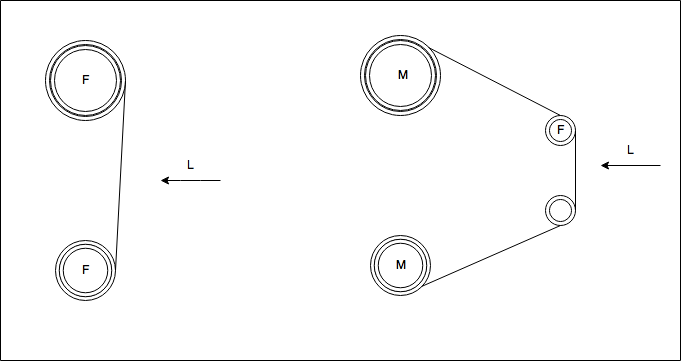
\includegraphics[scale=0.37]{esquema.png}
  \centering
  \caption{Femto before and after the mechanical modification. M is the print motor, F is the Faulhaber motor, and L is the laser beam.}
\end{figure}
 %%%%%%%%%%%%%%%%%%%%%%%%


\subsection{Reviewed Proposal}

% Ao estudar a dinamica do Femto mais a fundo, percebemos que poderiamos aprimorá-lo de outras maneiras. O modulo C-863 utilizado para o controle do motor era completamente subutilizado. Ele possui funcionalidades como controle de posicao, memoria interna, interface com joystick, controle de frenagem e diversas outras funcionalidades que nao sao necessarias no sistema Femto. Alem do mais, este modulo possui um preco de aproximadamente (PRECO). Percebemos que e possivel baratear consideravelmente o projeto atraves da substituicao do modulo por um circuito ponte H e controle PWM.
% Tambem incluimos no projeto a possibilidade de acionamento via Bluetooth. Apesar do Femto nao gerar raio-x em intensidade suficiente para ser considerado perigoso, achamos interessante a possibilidade de que o sistema Femto seja acionado sem a necessidade de ter um operador proximo a fonte de raio-x.
% Tambem acrescentamos ao escopo do projeto um sinal sonoro que alerta quando o sistema esta em operacao.

By further studying the dynamics of Femto, we realized that we could improve it in other ways. The C-863 module used for motor control was completely underutilized. It has features such as position control, internal memory, joystick interface, brake control and many others that are not necessary in the Femto system. Besides, this module has a price of approximately R\$3000,00 (600 euros). We found out that it is possible to decrease the price of the project considerably through the replacement of the module by a H-bridge circuit and PWM control. 
Also we included in the project the opportunity to drive via Bluetooth. Despite the fact that Femto does not generate sufficient x-ray intensity to be considered dangerous, we find interesting the possibility that the Femto system is operated without a person close to the x-ray source. We also added to the project scope a beep that alerts when the system is in operation.

% \section{System Design}
% This chapter describes the activities in the system design process. In this stage of the project, the IBM Rational Modeler software, version 7.5 \cite{IEEEhowto:IBM}, is  used for improvements in communication by specifying, visualizing and documenting the system, architecture and software designs.

% \subsection{Technical Requirements Definition}
% The Technical Requirements Definition Process transforms
% the stakeholder expectations into a definition of
% the problem and then into a complete set of validated
% technical requirements expressed as “shall” statements
% that can be used for defining a design solution for the future Product Breakdown Structure (PBS) model and related
% enabling products.

% So the system has [n] defined requirements, as shown in figure (1)


% \subsection{Requirements Traceability Matrix}
% In this section the complete and thorough traceability of the system requirements is presented, in order to ensure the impacts of any changes are fully assessed for all parts of the system.


\section{Targets : Schematics and Circuits}

% O motor utilizado \cite{IEEEhowto:motor} possui alimentacao 25V e um encoder com dois canais. Para esta etapa do projeto, utilizaremos apenas um canal do encoder para termos um feedback da velocidade.

The engine used \cite{IEEEhowto:motor} has power supply of 25V and an encoder with two channels. For this stage of the project we will use only one encoder channel to have a speed feedback.

%%%%%%%%%%%%%%%%%%%% Motor and Pot FIGURES %%%%%%%%%%%%%%%%%%%%
\begin{figure}[!ht]%{\linewidth}  
  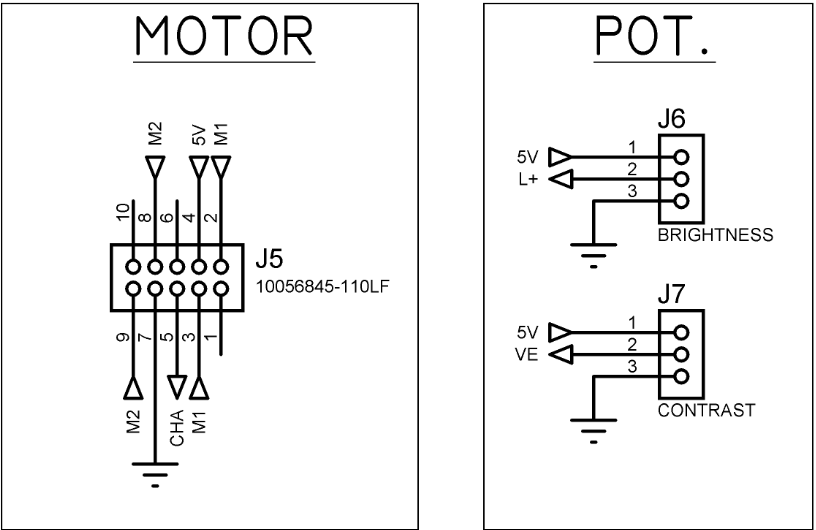
\includegraphics[scale=0.41]{motorPot.png}
  \centering
  \caption{Motor and Power Module Schematic Diagrams.}
\end{figure}
%%%%%%%%%%%%%%%%%%%%%%%% END OF FIGURE %%%%%%%%%%%%%%%%%%%%%%%%

%%%%%%%%%%%%%%%%%%%%%%%% H-Bridge FIGURE %%%%%%%%%%%%%%%%%%%%%%
\begin{figure}[!ht]%{\linewidth}  
  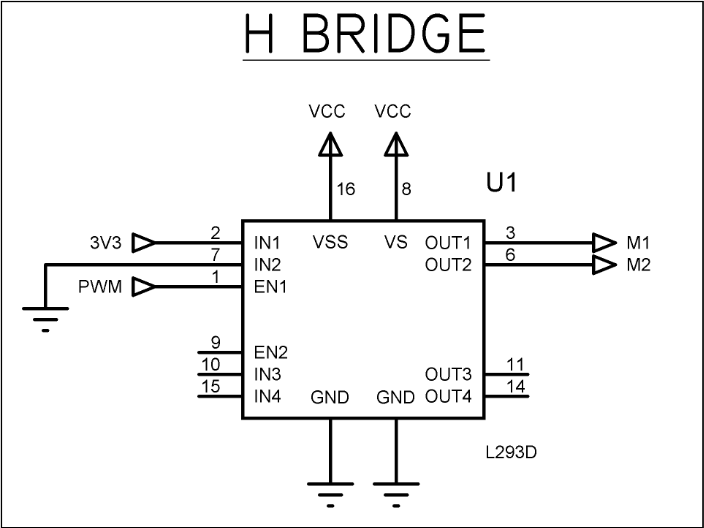
\includegraphics[scale=0.47]{hBridge.png}
  \centering
  \caption{H-Bridge Schematic Diagram.}
\end{figure}
%%%%%%%%%%%%%%%%%%%%%%%% END OF FIGURE %%%%%%%%%%%%%%%%%%%%%%%%

% O motor \cite{IEEEhowto:motor} e alimentado atraves de um circuito de ponte H \cite{IEEEhowto:L293D} chaveado atraves do controlador\cite{IEEEhowto:FRDM-KL25Z4} por um pulso PWM. Foi necessario utilizarmos um circuito divisor de tensao para adequar a tensao da fonte a faixa de tensao de trabalho do encoder.

The motor is powered through a H bridge circuit switched through the board by a PWM pulse. It is necessary a voltage divider circuit to adjust the voltage of the source to the encoder working voltage.

%%%%%%%%%%%%%%%%%%%% Voltage Divider FIGURE %%%%%%%%%%%%%%%%%%%
\begin{figure}[!ht]%{\linewidth}  
  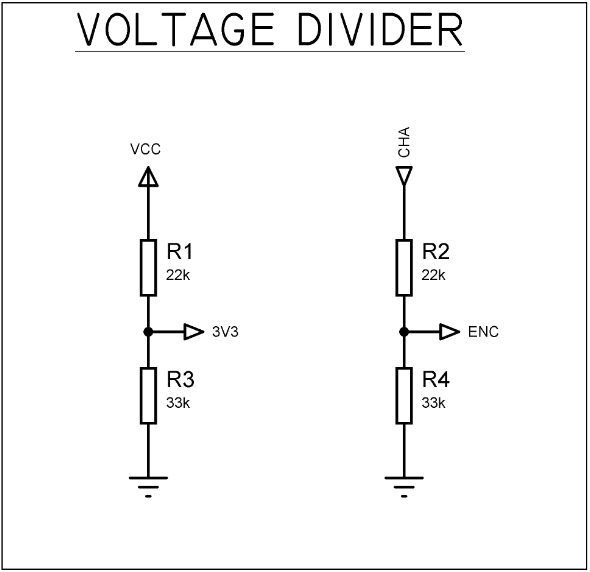
\includegraphics[scale=0.57]{voltageDivider.png}
  \centering
  \caption{Voltage Divider Schematic Diagram.}
\end{figure}
%%%%%%%%%%%%%%%%%%%%%%%% END OF FIGURE %%%%%%%%%%%%%%%%%%%%%%%%

% Para o modulo bluetooth \cite{IEEEhowto:bluetooth}, foi necessario um circuito regulador de tensao para manter a alimentacao estavel. As portas RX e TX do modulo foram ligadas as portas UART do microcontrolador. Atraves do aplicativo BlueTerm \cite{IEEEhowto:blueterm} conseguimos enviar e receber dados via comunicacao serial entre o modulo bluetooth e um celular Android

For the Bluetooth module \cite{IEEEhowto:bluetooth}, a voltage regulator circuit was necessary to maintain the stability of the power supply. The module’s RX and TX  ports were connected to the board’s UART ports. Through the BlueTerm \cite{IEEEhowto:blueterm} application was possible to send and receive data via serial communication between the Bluetooth module and an Android phone.

%%%%%%%%%%%%%%%%%%%%%%% Regulator FIGURE %%%%%%%%%%%%%%%%%%%%%%
\begin{figure}[!ht]%{\linewidth}  
  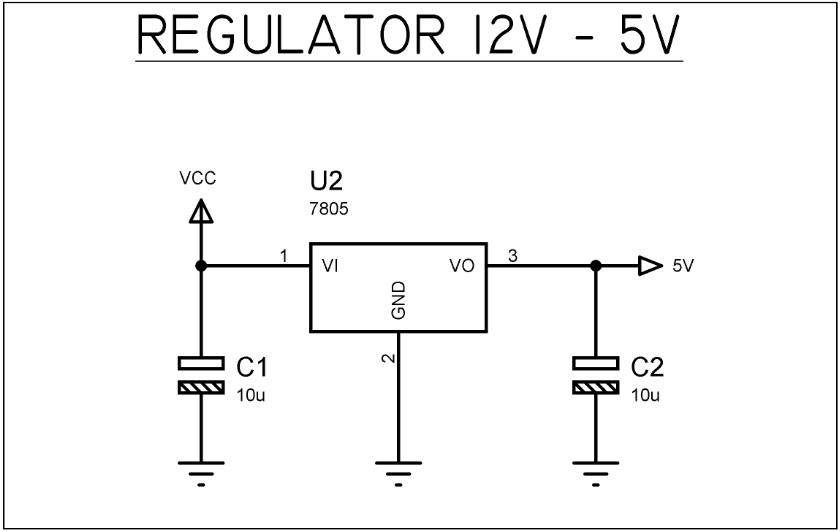
\includegraphics[scale=0.40]{regulator.png}
  \centering
  \caption{Regulator Schematic Diagram.}
\end{figure}
%%%%%%%%%%%%%%%%%%%%%%%% END OF FIGURE %%%%%%%%%%%%%%%%%%%%%%%%

%%%%%%%%%%%%%%%%%%%%%%%%% LCD FIGURE %%%%%%%%%%%%%%%%%%%%%%%%%%
\begin{figure}[!ht]%{\linewidth}  
  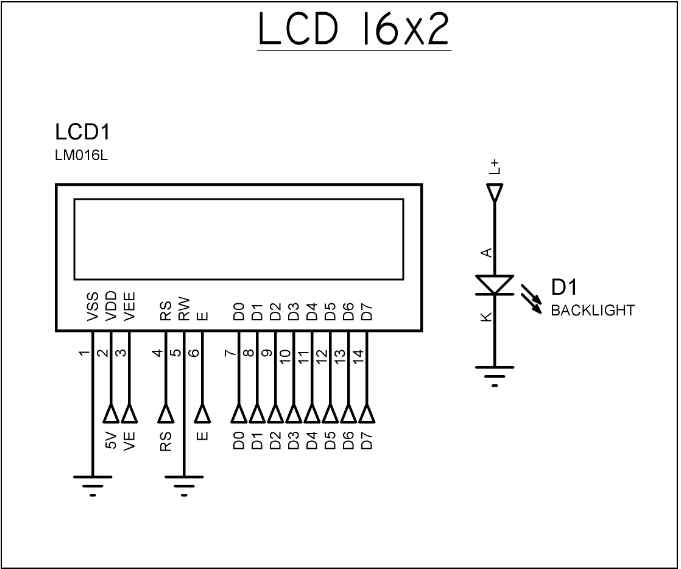
\includegraphics[scale=0.49]{lcd.png}
  \centering
  \caption{LCD Schematic diagram}
\end{figure}
%%%%%%%%%%%%%%%%%%%%%%%% END OF FIGURE %%%%%%%%%%%%%%%%%%%%%%%%

% Também foi utilizado um buzzer para servir de alarme quando o sistema entrasse em operação. O buzzer foi conectado diretamente no microcontrolador, com um diodo em antiparalelo para evitar retorno de corrente induzida pela sua bobina interna.

It has also been used a buzzer to serve as alarm when the system enters into operation. The buzzer was connected directly to the microcontroller, with a diode in antiparallel to avoid current return induced by its internal coil.

% Buscamos reaproveitar ao maximo os codigos desenvolvidos durante os laboratorios da disciplina para otimizar o trabalho. Assim, as portas usadas para cada periferico se assemelham as coneccoes dos perifericos utilizados em laboratorio.

We seek the maximum reuse of the codes developed during the laboratories to optimize the work. Thus, the ports used for each peripheral resemble the connections of peripherals used in the laboratory.

%%%%%%%%%%%%%%%%%%%%%% FRDM-KL25Z FIGURE %%%%%%%%%%%%%%%%%%%%%%
\begin{figure}[!ht]%{\linewidth}  
  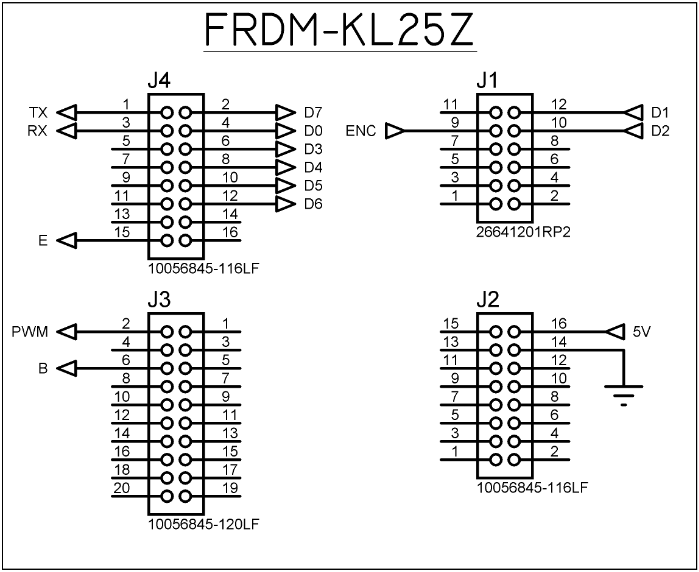
\includegraphics[scale=0.48]{frdmKL25Z.png}
  \centering
  \caption{FRDM-KL25Z4 Schematic Diagram.}
\end{figure}
%%%%%%%%%%%%%%%%%%%%%%%% END OF FIGURE %%%%%%%%%%%%%%%%%%%%%%%%


\section{Implementation}

% Usou-se o modulo bluetooth como UART (Universal Asynchronous Receiver Transmitter), usando o protocolo RS232 com boud rate de 9600 bps. O controlador interpreta os caracteres recebidos um a um. Os comandos são os seguintes:

We use the Bluetooth module as UART (Universal Asynchronous Receiver Transmitter) using the RS232 protocol with baud rate of 9600 bps. The controller interprets the received characters one by one. The commands are the following:


\begin{itemize}
\item VS: Start the system, powering the engine with PWM 100\%, triggering the LCD with the PWM frequency and angular speed of the motor and returning a beep indicating that the system is in operation
\item VC: Turn off the system.
\item VPxxx: Sets the speed from the value "xxx", which must be between the values 0 and 100 which indicates the \% of desired PWM for the motor)
\end{itemize}

% Em caso de erro, o sistema retorna atraves do Modulo Bluetooth "ERR", em caso de sucesso retorna "ACK". Utilizamos como interface o BlueTerm para Android, mas como pacos futuros, desejamos substituir esses comandos por uma interface mais amigavel.

% Utilizamos controle de velocidade pwm para o motor. O PWM e ligado a um CI de ponte H que tem a funcao de drive de potencia para o motor.

% Para aquisição da velocidade, utilizamos o encoder próprio do motor, com um dos seus canais conectado a placa conforme mostrado nas figuras da seção anterior.

% As funcoes necessarias para a comunicacao dos dados aquisitados para o display lcd estao anexas no arquivo "lcd\_hal.c".

% O circuito do buzzer e o mais simples. O buzzer e ligado e desligado, mantendo-se 1ms em cada estado, durante um segundo. Sua implementação pode ser encontrada nos arquivos "buzzer\_hal" e "tradutorUart", como podemos ver na matriz de rastreabilidade.

In case of error, the system returns through the Bluetooth module the message "ERR"; in case of success, the system returns the message "ACK". We used the BlueTerm application for Android as interface, but as future steps, we want to replace these commands for a more friendly interface.
We used PWM control of speed to the motor. The PWM is connected to an H-bridge IC that has the function of power drive to the motor.

For speed acquisition, we used the motor encoder itself, with one of its channels connected to a plate as shown in the figures of the previous section.
The necessary functions for the communication of the obtained data to the LCD display station are attached in the file "LCD\_hal.c".

The circuit of the buzzer is the simplest. The buzzer is turned on and off, keeping 1 [ms] in each state for a second. Its implementation can be found in the files "buzzer\_hal" and "tradutorUart", as we see in the traceability matrix.

\section{Problems and solutions}

\subsection{IDE Kinetis installation}

The first trouble with the project was the Kinetis IDE installation, once we tried to work with macOS X operational system. Nevertheless, the used debbuger indicated by Prof. Denis was not available for this operational system, and according to the Kinetis Design Studio's installation guide, the only option for macOS is the "Segger" debugger. At this moment we decided to move on Windows operational system in order to solve that problem.

On Windows platform we had also some problems with the installation. After KDS installation the option "Kinetis SDK 1.x project" was not available on "File $\rightarrow$ New" tab. The solution for this problem is the installation of the newest version of KDS software (version 3.2.0) instead of KDS version 3.0.0.

\subsection{LCD Display}

With the LCD display we had some difficulties to actuate on it, and after testing the code on the boards available in the laboratory at UNICAMP we realized that the code is made well. After some problems with the initially LCD installed (which was broken), we have installed a second one, which displays the angular velocity of the motor correctly.

\subsection{Bluetooth Module}

In the beginning the Bluetooth module was not very stable, and it was hard to have a connection between the Android system and the Bluetooth module for more than some seconds. We studied some possible answers for this scenario, which bring us to the problem with the stability of the voltage supply source. Therefore a regulator 12 [V] - 5 [V] was connected to the circuit in order to supply the Bluetooth, fixing the problem.

\subsection{Motor Results}

When acting on the motor by PWM, we figured out that the motor angular velocity was not linear concerning the PWM duty cycle. We currently investigate 2 hypothesis for this problem : first, that the used H-Bridge (L293D) \cite{IEEEhowto:L293D} may have a switching frequency lower than the PWM one. Second, that the motor output may be not linear.
%Tem que TODO isso ainda.

\section{Future Project Steps}

Since Femto is a big project, it continues to be developed in order to apply some improvements to it. The next steps for the project are: 

% O Femto e um projeto em construcao e continuaremos trabalhando para aprimora-lo. Para tal planejamos algumas melhorias:


\begin{itemize}
%    \item Substituicao do modulo bluetooth por um modulo wifi e integracao com um sistema de cameras que permitiria que o experimento fosse monitorado a distancia. Para tal também seria necesario a imprementacao de um servidor e uma GUI para computador e/ou mobile.
\item Substitution of the Bluetooth module for WiFi module and integration with a camera system that would allow the experiment to be monitored from any place with internet connection. To do this improvement in the system, it will also be necessary to implement a server and a GUI for computer and/or mobile.
%    \item Sistema de fim de curso para detectar quando o rolo da fita alvo de titanio chegar ao fim e implementacao de rotina de inversao mais paco do motor. A primeira hipotese e que esta deteccao seja feita atraves de sensor otico.
\item Limit system to detect when the roll of titanium target tape reaches the end and engine inversion routine implementation. The first hypothesis is that this detection will be done through an optic sensor.
%    \item Refinar o controle de velocidade e tensao mecanica da fita atraves de controladores PID.
\item Refine tape's speed control and mechanical tension control through PID controllers.
\end{itemize}


\section{Conclusion}

% Tivemos a oportunidade de trabalhar em um projeto com aplicacao direta para a producao cientifica da Unicamp, melhorando a interface e seguranca satisfatoriamente. Alem do mais, conseguimos baratear consideravelmente o equipamento, trazendo ganhos para o laboratorio de pesquisa.

We had the opportunity to work on a project with direct application to the scientific production of UNICAMP, improving the interface and security satisfactorily. Besides, we were able to considerably cheapen the equipment, bringing gains for the laboratory research.

% Alem do mais, pudemos notar o quao relevante a modelagem de sistemas e para um projeto, pois pudemos facilmente reutilizar funcoes e codigos das atividades de laboratorios. Em projetos de engenharia, esta flexibilidade proporcionada por uma boa modelagem permite economizar esforcos e dinheiro, alem da facilidade de manutencao.

Besides, we noted how the relevant modeling systems are to a project, since we could easily reuse functions and codes of laboratories activities. In engineering, this flexibility afforded by a good modeling allows us to save efforts and money, besides the ease of maintenance.


\appendices
\section{Board Layout}

% Abaixo temos o layout da placa que sera fabricada para implementacao no Femto, contendo entradas para os perifericos utilizados e para o microcontrolador.

Below is the layout of the board that will be made for implementing in the Femto containing entries for the used peripherals and microcontroller.

%%%%%%%%%%%%%%%%%%%%% Board Layout FIGURE %%%%%%%%%%%%%%%%%%%%%%
\begin{figure}[!ht]%{\linewidth}  
  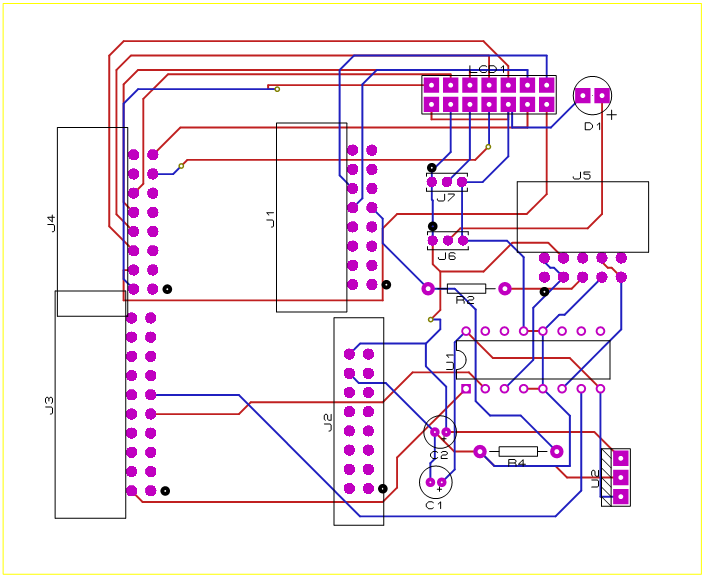
\includegraphics[scale=0.49]{boardLayout.png}
  \centering
  \caption{Created Board Layout Schematic Diagram.}
\end{figure}
%%%%%%%%%%%%%%%%%%%%%%%% END OF FIGURE %%%%%%%%%%%%%%%%%%%%%%%%


% use section* for acknowledgment
\section*{Acknowledgment}

This work is the result of a Embedded Systems Laboratory Project at UNICAMP - University of Campinas in Campinas, S\~{a}o Paulo, Brazil, guided by Prof. Denis S. LOUBACH \cite{IEEEhowto:denis}.

The authors would like to thank to UNICAMP for the opportunity to acquire experience in research and development, and their Prof. Denis S. LOUBACH for the guidance,  all support during all steps of the project and relevant discussions that helped the authors in the process of understanding, analyzing and correcting various problems of the project.


% Can use something like this to put references on a page
% by themselves when using endfloat and the captionsoff option.
\ifCLASSOPTIONcaptionsoff
  \newpage
\fi



\begin{thebibliography}{1}

\bibitem{IEEEhowto:denis}
LOUBACH,~D.~S., \emph{Lecture Notes of the course ES670 - Embedded Systems Theory and Laboratory}, 2016.\hskip 1em plus
  0.5em minus 0.4em\relax Virtual Environment MOODLE of UNICAMP, Brazil.
  
\bibitem{IEEEhowto:FRDM-KL25Z4}
NXP Semiconductors - Freedom KL25Z4 Data-sheet Board.

\bibitem{IEEEhowto:Bremmsstrahlung}
Eberhard Haug \& Werner Nakel (2004). The elementary process of bremsstrahlung. River Edge NJ: World Scientific. p. Scientific lecture notes in physics, vol. 73. ISBN 981-238-578-9.

\bibitem{IEEEhowto:motor}
FAULHABER DC-Micromotor Serie 2230 024 S.

\bibitem{IEEEhowto:PI}
MERCURY C-863 DC CONTROLLER - PI.

\bibitem{IEEEhowto:Kinetis}
NXP Semiconductors - Kinetis Design Studio Integrated Development Environment (IDE).

\bibitem{IEEEhowto:IBM}
IBM Rational Rhapsody Modeler 7.5.

\bibitem{IEEEhowto:L293D}
L293D QUADRUPLE HALF-H DRIVERS - Texas Instruments.

\bibitem{IEEEhowto:bluetooth}
BLUETOOTH MODULE RS232 HC-05.

\bibitem{IEEEhowto:blueterm}
BLUETERM App for Android - pymasde.es.

\end{thebibliography}

\end{document}